\documentclass[../../main.tex]{subfiles}
\begin{document}

\subsection*{7.10}
Un filo metallico rigido di forma qualunque ha due estremi c e n che possono scorrere senza attrito su due rotaie orizzontali distanti $d = 20\ cm$.
\\Le rotaie sono poste in un campo magnetico $B = 0.5\ T$ uniforme e verticale.
\\Il cicuito è percorso da una corrente costante $i = 2A$ fornita dal generatore G.
\\Se la massa del filo è m=2g calcolare la velocità v del filo e lo spazio x percorso dopo un tempo $t_1 = 0.15$, nell'ipotesi t=0 il filo sia fermo.
\\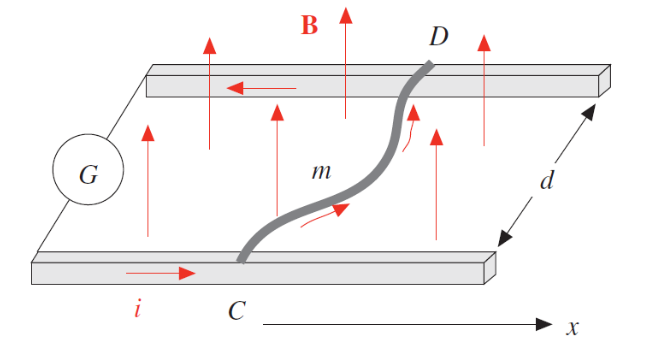
\includegraphics[scale=0.3]{e_7_10_0.png}
\\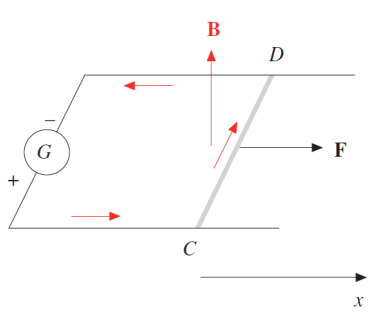
\includegraphics[scale=0.3]{e_7_10_1.png}
\subsubsection*{Formule utilizzate}
\subsubsection*{Soluzione punto a}
$\vec{F} = i\int_C^D d\vec{s}\wedge\vec{B} = i\vec{CD}\wedge\vec{B} = iBd\vec{u_x}$
\\$v= \frac{iBd}{m}t_1 = 10 frac{m}{s}$
\\$x=\frac{1}{2}\frac{iBd}{m}t_1^2=0.5\ m$
\subsubsection*{Soluzione punto b}
\newpage

\end{document}